\chapter{Theoretische Grundlagen}
\label{chap:theoretische_grundlagen} Dieses Kapitel führt in die theoretischen Grundlagen
ein, die in dieser Arbeit benötigt werden. Den ersten Teil bilden die domänenspezifischen
Grundlagen \ref{sec:domänenspezifisch}, welche genauer darauf eingehen, welchen Inhalt
die zu bearbeitenden Bilder bieten und wie dieser zu verstehen ist. Abschnitt
\ref{sec:technologisch} geht hierbei auf verschiedenen Technologien ein, die eine
wichtige Rolle spielen. Der Abschnitt \ref{sec:verwwandte_arbeit} geht auf die
Arbeit von \citet{hoffmann2020} ein und legte damit den Grundstein dieser Arbeit.
Die Abschnitte \ref{sec:3d_slicer} und \ref{sec:architektonisch} führen in
Softwareentwicklungsthemen ein, die zum Erstellen einer \textit{3D Slicer
Extention} wichtig sind.
% ---------------------------------------------------------------------------------------

\section{Domänenspezifisch}
\label{sec:domänenspezifisch} Wie bereits aus dem Kapitel \ref{chap:einleitung}
Einleitung klar wurde, handelt es sich bei den Micro-CT Bilder um Zahnbilder,
die aufgrund von Zahnkaries entfernt wurden. Um zu verstehen, wie eine CT-Aufnahme
eines Zahns aufgeteilt werden soll, ist es hilfreich zu verstehen, wie ein Zahn
aufgebaut ist.

\begin{minipage}{0.40\textwidth}
	Die Abbildung \ref{fig:aufbau_eines_zahnes} zeigt den groben Aufbau eines Zahnes
	nach \citet[Seite 17]{lehmann2012Zahnheilkunde}. Zu sehen ist, dass das Denit oder
	auch Zahnbein genannt, den Großteil eines Zahnes einnimmt. Im Bereich der Zahnkrone
	wird das Dentin von Zahnschmelz überzogen. Der Zahnschmelz ragt in die
	Mundhöhle und ist nach \cite[Seite 41]{lehmann2012Zahnheilkunde} das härteste
	Material im menschlichen Körper. In der Mitte des Zahnes befindet sich Weichgewebe,
	welches als Pulpa bezeichnet wird vgl. \citep[Seite ]{lehmann2012Zahnheilkunde}.
\end{minipage}
\hfill
\begin{minipage}{0.50\textwidth}
	\centering
	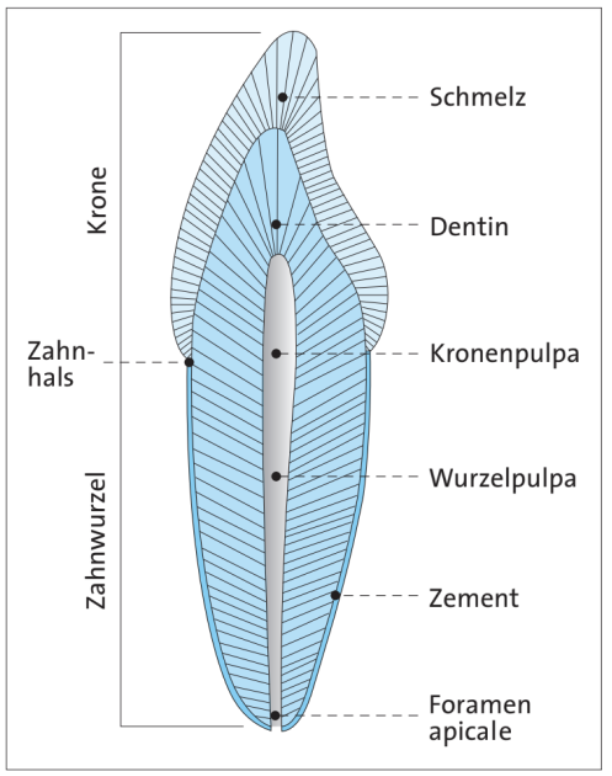
\includegraphics[scale=0.50]{img/aufbau_eines_zahns.jpg}
	\captionof{figure}{Aufbau eines Zahnes nach \citet{lehmann2012Zahnheilkunde}} \label{fig:aufbau_eines_zahnes}
\end{minipage}

Für die Bearbeitung von Micro-CT Aufnahmen sind die Bereich Schmelz Dentin und Pulpa
von besonderer Bedeutung. Betrachtet man eine CT wie es zu Beginn in der
Abbildung \ref{fig:ct_aufnahme_eines_zahns} gezeigt wurde, so bilden diese 3 Gewebearten
die unterschiedlichen Grauwerte in einem CT-Bild. \\ \textbf{Pulpa:} Die Pulpa unterscheidet
sich hierbei nur wenig vom Hintergrund, da sie als einzige der drei Hauptteile
eines Zahnes ein Weichgewebe ist und bei einer Röntgenaufnahme nicht absorbiert.
Geht man weiter von innen nach außen, so ist der nächste Zahnteil auf einem CT
das Zahnbein. \\ \textbf{Dentin:} Das Dentin ist laut \citet[Seite 41]{lehmann2012Zahnheilkunde}
eine Hartsubstanz, die dem Kieferknochen sehr nah steht. So kommt es, dass dieser
Teil schon deutlich besser auf einem CT zu erkennen ist. Den äußersten Teil in
der Mundhöhle bildet das Zahnschmelz. \\ \textbf{Schmelz:} Der Schmelz ist wie
bereits erwähnt, der härteste Teil im menschlichen Körper und aus diesem Grund auch
am hellsten auf dem CT zu erkennen. Die folgende Abbildung
\ref{fig:pulpa_dentin_schmelz} sollen durch Gegenüberstellung den Zusammenhang
zwischen einem CT-Bild und einer Zahnzeichnung verdeutlichen.

\begin{figure}[h]
	\centering
	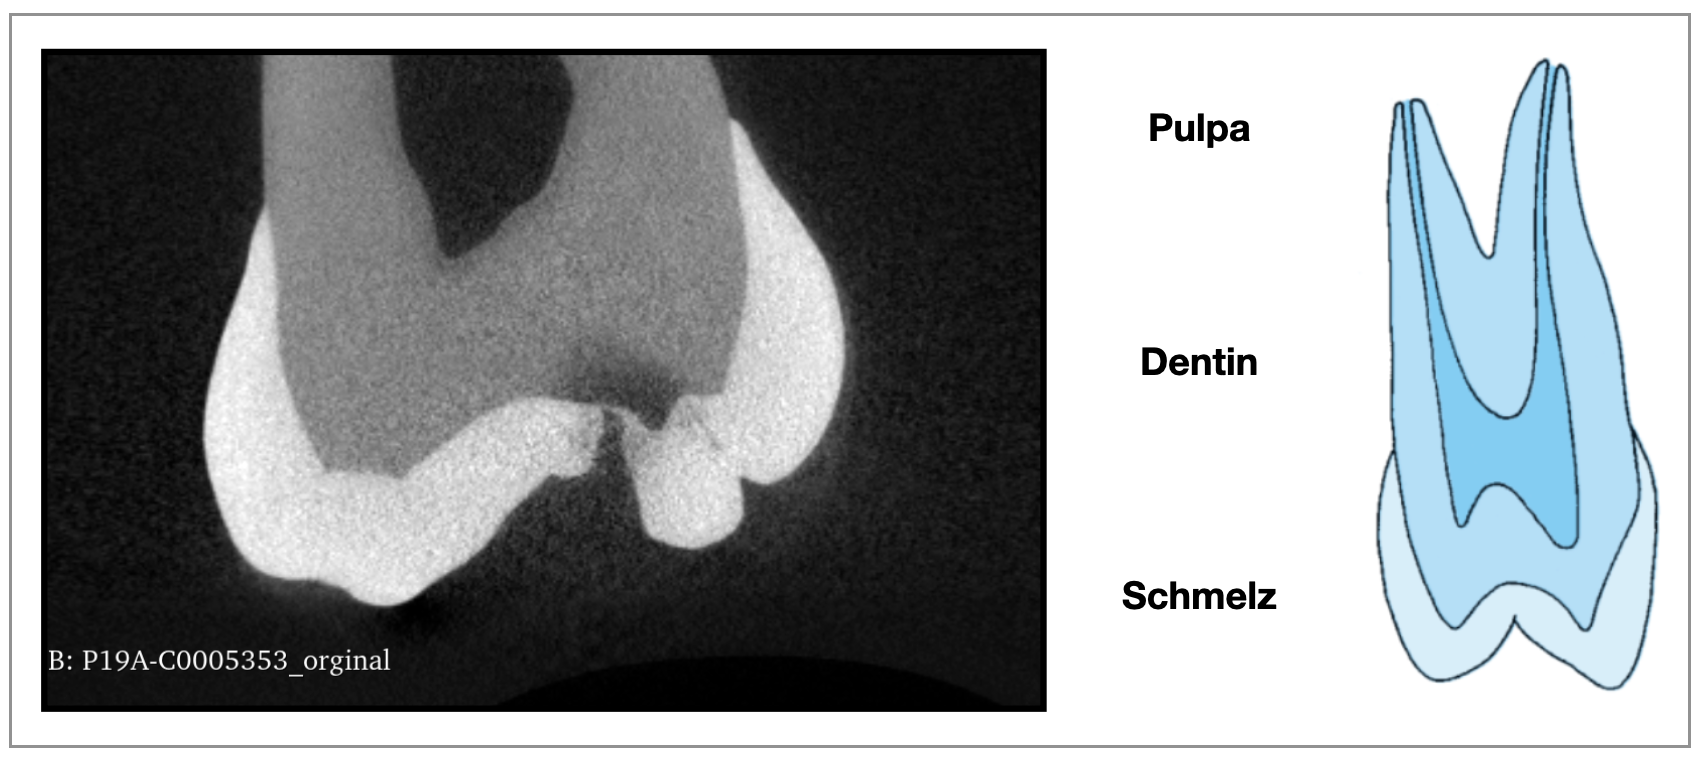
\includegraphics[width=0.9\textwidth]{
		img/Bildschirmfoto 2024-11-22 um 15.13.24.jpg
	}
	\caption{Darstellung von Pulpa, Dentin und Schmelz auf einer CT-Aufnahme (link)
	und einer Zeichnung (rechts) nach \citet[Seite 29]{lehmann2012Zahnheilkunde}. }
	\label{fig:pulpa_dentin_schmelz}
\end{figure}

Mit diesem Domänenwissen kann ein Schritt weiter gegangen werden, sodass der
Fokus nun auf die CT-Bilder gesetzt wird. Das Kapitel \ref{sec:technologisch} Technologien
führt die Technologie der Computertomografie tiefer ein. Mit diesem
Domänenwissen kann ein Schritt weiter gegangen werden, sodass der Fokus nun auf die
CT-Bilder gesetzt wird. Das Kapitel \ref{sec:technologisch} Technologien führt
die Technologie der Computertomografie tiefer ein.
% ---------------------------------------------------------------------------------------

\section{Bildgebung}
\label{sec:technologisch} Es gibt die unterschiedlichsten Arten zur Erzeugung
dreidimensonaler Bilddaten. Dieser Abschnitt erläutert federführend die Technologie
der Micro-CT Aufnahmen und deren Erstellung. Diese sind für eine medizinischen
Einsatz besonders interessant. Des Weiteren erfolgt eine Einführung in die Speicherung
und Komprimierung von CT-Aufnahmen. Dies sorgt dafür, dass die digitalen Bilddaten
deutlich handlicher werden.
% ---------------------------------------------------------------------------------------

\subsection{Computertomografie}
\label{subsec:computertomografie} Die Erfindung der Computertomografie (CT) war ein
Quantensprung in der Geschichte der Medizin. Sie ist aus heutigen Diagnosen
nicht mehr wegzudenken. Ein Micro-CT Bild ist laut \citet[Abstract]{baird2017} ein
Menge hochauflösender Bilder, die wie ein Stapel zusammengelegt werden. Der Aspekt
Micro deutet dabei darauf hin, dass es eine miniaturisierte Ausführung eines
üblichen Kegelstrahl-CTs ist so \citet[Seite 340]{buzug2011}. Eine andere Definition
erläutert \citet{lehmann2013bildverarbeitung}. Er beschreibt die Computertomografie
als Projektionen einzelner Ebenen im Untersuchungsobjekt. Die Technologie, mit der
diese Bilderstapel aufgenommen werden, ist unter der Röntgentechnik oder auch X-Ray
bekannt. Die Röntgenstrahlung ist eine Form der elektromagnetischen Strahlung,
ähnlich wie das sichtbare Licht so das \citet{nib2024}. Anders als das Licht
haben die Röntgenstrahlen eine viel höhere Energie. Das führt dazu, dass man mit
dieser elektromagnetischen Strahlung viele Objekte durchdringen kann. So auch Gewebeteile
eines Zahnes vgl. \citep{nib2024}. Die Abbildung \ref{fig:spectrum} zeigt diese
elektromagnetische Spektrum.

\begin{figure}[h]
	\centering
	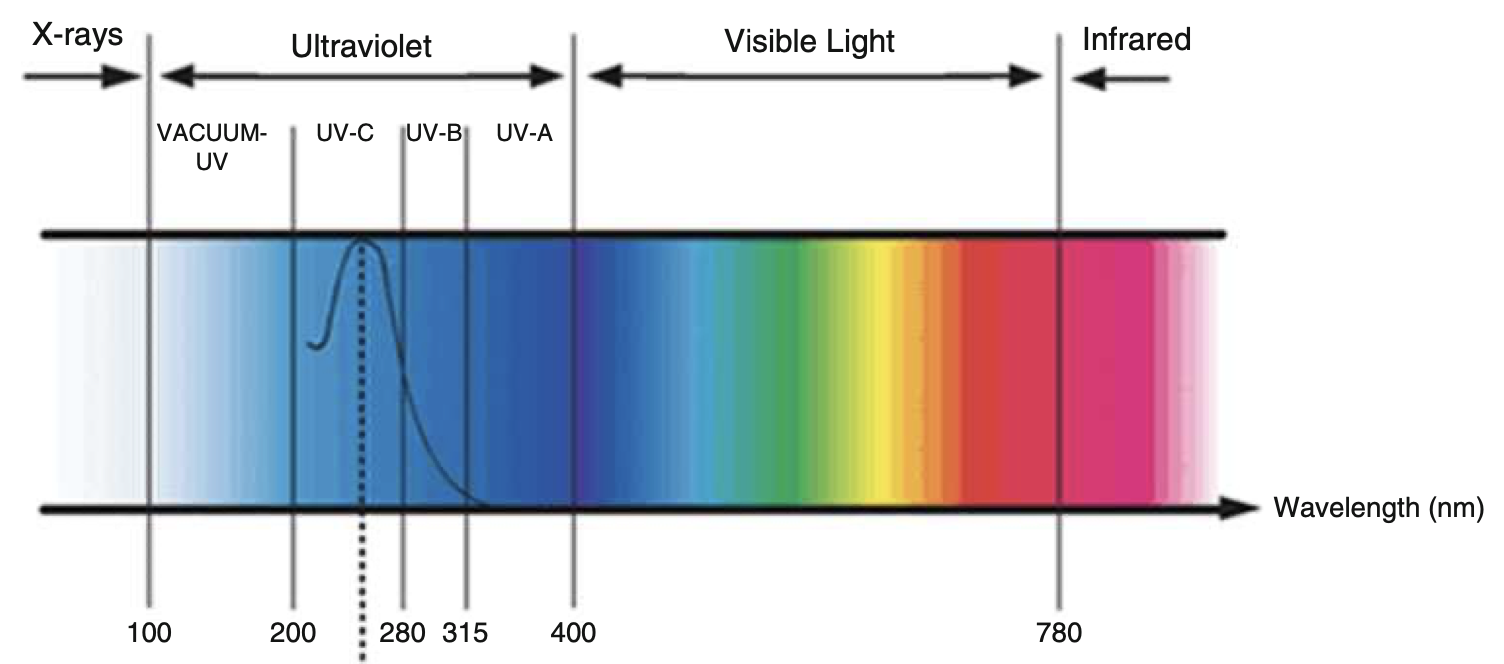
\includegraphics[width=0.6\textwidth]{img/x_ray.jpg}
	\caption{Einordnung der Röntgenstrahlung (X-Ray) nach dem \citet{zwinkels2015}}
	\label{fig:spectrum}
\end{figure}

Durchdringt ein solcher Röntgenstrahl ein Untersuchungsobjekt, werden die
Details aufgrund der Wechselwirkung mit Materie auf einer CT-Probe sichtbar. Die
bekannteste Wechselwirkung ist die Absorption. Mit der Steigerung der Atomzahl
in einem Material nimmt auch die Absorption eines Materials zu, sodass es leicht
ist verschiedenen Materialien in einer CT-Aufnahme zu unterscheiden \citep[vgl.][]{nib2024}.

Für eine Micro-CT Aufnahme bedarf es spezieller Technik. Es gibt unterschiedliche
Firmen, welche die unterschiedlichsten Modelle anbieten. Im Falle der Zahnklinik
an der LMU in München handelt es sich um ein Micro-CT 40 der Firma \citet{scanco2024}.
Dieses Gerät erstellt Aufnahmen mittels Röntgenstrahlung und generiert mithilfe der
Computertomografie ein dreidimensionales Bild, welches im Format \texttt{.ISQ} abgelegt
wird. Wie das nächste Kapitel beschreiben wird, ist der Speicherumfang den solch
ein Bild benötigt, deutlich zu groß. Es bedarf einer Technik, mit der die
Aufnahmen auf eine handhabbare Größe schrumpfen.
% ---------------------------------------------------------------------------------------

\subsection{Datensätze}
\label{subsec:datensätze} Die rohen Datensätze, welche direkt aus dem Micro-CT Gerät
kommen, haben nach \citet{scanco2024} das Format \texttt{.ISQ}. Dieses Format fällt
speziell auf die Geräte der Firma SCANCO zurück. Wie das vorherige Kapitel
\ref{subsec:computertomografie} bereits eingeführt hat, ist dieser Dateityp für eine
weitere Bearbeitung nicht geeignet. Unter anderem wegen ihrer Größe. \citet{RoeschKunzelmann2018}
haben hierfür ein Paket entwickelt. Dieses konvertiert ein \texttt{.ISQ} Format
in ein \texttt{.mhd} Format. Bei einer \texttt{.mhd} Datei handelt es sich um ein
Metafile, dass auf die eigentliche Datei verweist. Folgender Ausschnitt zeigt die
Verwendung des Pakets.

\texttt{python3 isq\_to\_mhd.py <quelle> <ziel>}

Diese Meta-Datei kann genutzt werden, um interessante Informationen über das
Bild zu erlangen. Wird dieses Kommando ausgeführt, so erstellt das Skript
\texttt{isq\_to\_mhd} ein Metafile, das detailliert Daten über die Datei enthält.
Ein Ausschnitt dieses Metafiles liefer das Listing \ref{lst:inhalt_mhd_datei}

\begin{lstlisting}[
	caption={Ausschnitt des Inhaltes einer MHD-Datei},
	label={lst:inhalt_mhd_datei}]
ObjectType = Image
NDims = 3
CenterOfRotation = 0 0 0
ElementSpacing = 0.02 0.02 0.02
DimSize = 1024 1024 517
ElementType = MET_SHORT
ElementDataFile = P01A-C0005278.ISQ
\end{lstlisting}

In der Datei sind Informationen über die Ausprägung, Art und Größe der Datei zu
finden. Besonders interessant sind die Punkte \texttt{DimSize und ElementType}. Über
diese Parameter lässt sich die Größe eines Bildes berechnen. \citet[Seite 10-11]{burger2009}
erklärt, das ein Bild in Zellen aufgeteilt ist, welche Informationen enthalten. Diese
Zellen sind im zweidimensionalen Raum als Pixel bekannt. Betrachtet man jedoch
ein, wie im Falle der Zahnklinik an der LMU dreidimensionales Bild, so spricht
man nicht mehr von einem Pixel, sondern von einem Voxel. Ein Voxel ist demnach
das dreidimensionale Äquivalent zu einem Pixel. \citet[Seite 10-11]{burger2009} beschreibt
weiter das jeder diese Zellen ein binäres Wort der Länge $2^{k}$ ist. Die Basis
2 ergibt sich durch das binäre Wort, wo hingegen für $k$ gilt:
$k \in \mathbb{N}$. Um für den konkreten Fall aus Listing \ref{lst:inhalt_mhd_datei}
das entsprechenden $k$ zu ermitteln, muss der \texttt{ElementType} näher betrachtet
werden. \texttt{MET\_SHORT} steht hierbei für Signed short, was eine Größe von
16 Bit entspricht. Damit ergibt sich für die Länge $k$ ein Wert von 4. So können
nach \citet[Seite 10-11]{burger2009} folgende Gleichungen festgehalten werden.

\begin{align}
	\label{equ:größe_bestimmen}1024 \cdot 1024 \cdot 517    & = 542,113,792 \, \text{Voxel}\notag  \\
	542,113,792 \, \text{Voxel}\cdot 2 \, \text{Byte/Voxel} & = 1,084,227,584 \, \text{Byte}\notag \\
	1,084,227,584 / 1,000,000,000                           & = 1.0842 \, \text{GB}
\end{align}

Die erste Gleichung bestimmt die Gesamtzahl aller Voxel in einem Bild. Gleichung
2 ermittelt die Größe des Bildes in der Einheit Byte. Die letzte Zeile nimmt
eine Umrechnung von Byte nach Gigabyte (GB) vor.

Durch die Gleichungen in \ref{equ:größe_bestimmen} wird klar, das eine CT-Aufnahme
des Typs \texttt{.ISQ} direkt nach seiner Aufnahme über einen GB groß ist. Laut \citet{poliklinikLMU}
ist dies ein zu großes Format. Es stellt sich also die spannende Frage, wie
solch eine Datei komprimiert werden kann, ohne das es Verluste in der Qualität gibt.
Dr. Elisa Walter hat hierfür eine Lösung entwickelt. QUELLE Betrachtet man den
\texttt{ElementType} genauer, so fällt auf, dass es noch weiter Typen gibt, die
durch eine geringere Länge $k$ deutlich weniger Speicher benötigen. Durch Anwendung
simpler Statistik lässt sich herauslesen, das die $2^{4}$ Byte je Element nicht
ausgenutzt werden. Als Werkzeug für die Betrachtung einer solchen Statistik kann
das Histogramm eines Bildes genutzt werden. Laut \citet[Seite 249]{jahne2024}
ist ein Histogramm die Häufigkeitsverteilung der Grauwerte. Diese zeigt Grafisch
die unterschiedlichen Grauwerte (X-Achse) zu ihren Häufigkeiten im Bild (Y-Achse).
\citet[Seite 249]{jahne2024} macht deutlich, dass das Histogramm jedoch kein AUfschluss
über die räumliche Verteilung der Pixel oder Voxel liefert. Werden einige der
Argumente nicht verwenden, so kann der \texttt{ElementTyp} verkleinert werden
% ---------------------------------------------------------------------------------------

\section{Bildbearbeitung}
\label{sec:bildbearbeitung} Nachdem ein CT erzeugt und gegebenenfalls komprimiert
wurde, verarbeitet werden. Für eine weitere Verarbeitung der Micro-CT Bilder bietet
das Pipeline-Modell von \citet[Seite 50]{handels2000} eine gute Richtlinie. Er
beschreibt mit dieser Visualisierungs-Pipeline Schritte, die bei der Bearbeitung
und dreidimensionalen Darstellung von CT-Aufnahmen notwendig sind \citep[vgl.][Seite
50]{handels2000}. Die ersten Schritte, \textit{Bildvorverarbeitung} und \textit{Segmentierung},
sind von besonderem Interesse. Dieser Abschnitt orientiert sich an dieser Unterteilung
und nimmt sie als Vorbild. Daraus ergeben sich die Abschnitte
\ref{subsec:filter} Filter und \ref{subsec:segmentierung} Segmentierung.
% ---------------------------------------------------------------------------------------

\subsection{Filter}
\label{subsec:filter} CT-Aufnahmen rauschen, dies ist ein Fakt und liegt in der Natur
einer Röntgenaufnahme. Dies beschreiben auch \citet[Kapitel 3]{diwakar2018} in
ihrem Paper über CT-Bildrauschen und Entrauschen. Dabei liegt die Ursache des Rauschens
nicht an einer Stelle sondern ist auf viele Quellen zurückzuführen. Einen gute
Einteilung dieser Quellen liefern ebenfalls \citet[Kapitel 3]{diwakar2018}. Sie teilen
die Rauschquellen auf in \textit{Random noise, Statistical noise, Electronic
noise und roundoff noise}.

Unter dem Rauschen eines Bildes versteht man die Streuung der Pixelwerte im Bild.
Für eine Segmentierung des Bildes ist dieses Verhalten unerwünscht und führt zu schlechten
Ergebnissen \citep[vgl.][Seite 51]{handels2000}. Die Bildvorverarbeitung oder
auch Filter gennant, hat die Aufgabe dieses Rauschen so gut wie möglich zu redzieren.
Hierzu gibt es diverse Möglichkeiten.

\begin{minipage}{0.40\textwidth}
	Mit Blick auf die folgenden Kapitel sind für diese Arbeit vorallem die lokalen
	Operatoren relevant. Die lokalen Operatoren sind charakteristisch für die
	Betrachtung der lokalen Nachbarschaft. Jeder Pixel betrachtet also seine Umgebung
	und führt auf Basis darauf eine Berechnung des jeweils betrachteten Pixels durch
	\citep[vgl.][Seite 52]{handels2000}.
\end{minipage}
\hfill
\begin{minipage}{0.50\textwidth}
	\centering
	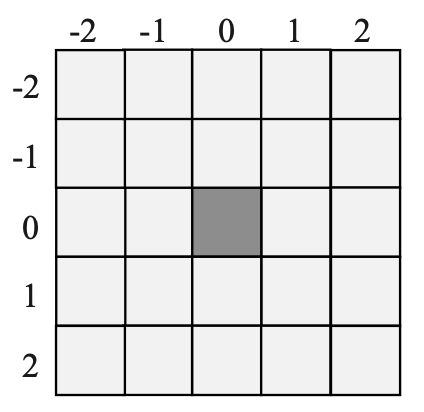
\includegraphics[width=0.60\textwidth]{img/lokaler_operator_maske.jpg}
	\captionof{figure}{Maske eines lokalen Operators nach \citet[Seite 52]{handels2000}}
	\label{fig:lokaler_operator_maske}
\end{minipage}

Für die konkrete Betrachtung der Nachbarschaft eines Pixels empfiehlt \citet[Seite
52]{handels2000} eine konkrete Maske (Ausschnitt) herranzuziehen, die mit einer
Matrix interpretiert werdenen kann und die Nachbarschafft eines Pixels abdeckt. Abbildung
\ref{fig:lokaler_operator_maske} zeigt eine sollche Maske und soll das Verfahren
so verdeutlichen. Der grau hinterlegte Mittelpunkt ist das aktuell betrachtete
Pixel. die Felder um die Mitte herum die Nachbaren. Es fällt jedoch auf, dass durch
dieses Schema nicht jede mögliche Ausprägung einer Maske in frage kommt. Um ein
Mittelpunkt und damit einen aktuellen Pixel betrachtetn zu können, bedarf es einer
ungeraden Seitenanzahl. Diese eingränzung lässt sich wie folgt generisch fassen.

\begin{align}
	\label{equ:lokaler_operator}M_{(2_m+1)x(2_m+1)} & = \begin{bmatrix}n & n & n & n & n\\ n & n & n & n & n\\ n & n & x & n & n\\ n & n & n & n & n\\ n & n & n & n & n\\\end{bmatrix}
\end{align}

Die Gleichung \ref{equ:lokaler_operator} beschreibt die mögliche Ausprägung eines
lokalen Operators als Matrix. Dabei sei $m \in \mathbb{N}$. Die Variable $x$ beschreibt
das aktuell betrachtete Pixel, während $n$ die Nachbarn illustrieren soll. Durch
die Gleichung ist auch zu erkennen, das die Maske des lokalen Operators beliebig
groß werden kann. Eine hohe Ordnung der Operatormatrix ist jedoch nicht immer von
Vorteil, sodass es letzten Endes auf den Anwendungsfall ankommt.

Mit der Technik der lokalen Operatoren können nun unterschiedliche Arten
angwenden werden. \citet[Seite 54 - 55]{handels2000} unterscheidet hier in Glättungsfilter,
Mittelwertfilter, Medianfilter, Gaußfilter und Binomialfilter. Alle dieser Filter
bedienen sich einer Operatormaske um auf Basis der Nachbarelementen ein Statistischen
Wert für den Bildpunkt zu erhalten. Um einen genaueren Einblick in alle Filter
zu erlangen, sei an dieser Stell auf \citet[Seite 54 - 55]{handels2000} verwiesen.

Wie zu Anfang dieses Kapitels beschrieben, ist eine Bildvorvearbeitung (Filterung)
für eine gute Segmnetierung des Bildes unerlässlich. So kommt es das auch in der
Visualisierungs-Pipelin nach \citet[Seite 50]{handels2000} der zweite Schritt bereits
die Segmentierung einführt. Warum dies so ein wichtiger Bestandteil der
Bildanalyse ist und welche Methoden sich hier bieten, erläutert das folgende Kapitel.
% ---------------------------------------------------------------------------------------

\subsection{Segmentierung}
\label{subsec:segmentierung} Die Bildsegmentierung oder Bildaufteilung ist ein wichtiges
Teilgebiet der Bildverarbeitung und beschäfftigt sich mit der Bildanalyse. Ihr
Ziel ist es, detailirtere beschreibende Bilder aus dem vorliegenden Orginalbild zu
berechnen. Dies kann im Falle eines CTs in der Zahnklinik an der LMU München die
hervorgehobene Darstelllung der Zahnhartsubstanzen sein. \citep[vgl.][Seite 359]{lehmann2013bildverarbeitung}.
Konkret teilt ein Segmentierungsverfahren also ein Bild in Teilbereiche auf. Dabei
sind die Teilbereich in sich bemerkenswert homogen. \citet[Seite 1]{ramesh2021}
beschreibt, dass der Prozess der Segmentierung zur Gewinnung wichtiger Informationen
dient wie zum Beispiel die Zahnkaries Ausbreitung. So kommt es, dass \citet[Seite
50]{handels2000} in seiner Visualisierungs-Pipelin die Segmentierung als zweiten
Schritt und damit als zentrales Problem darstellt.

\citet[Seite 95]{handels2000} und \citet[Seite 360]{lehmann2013bildverarbeitung}
beschreiben beide, dass die Bildsegmentierung eines CTs für eine gute und
eindeutige Ärzliche Diagnose nicht mehr wegzudenken ist. Warum dem so ist verdeutlicht
die Abbildung \ref{fig:interpretation_einer_ct_aufnahem}.

\begin{figure}[h]
	\centering
	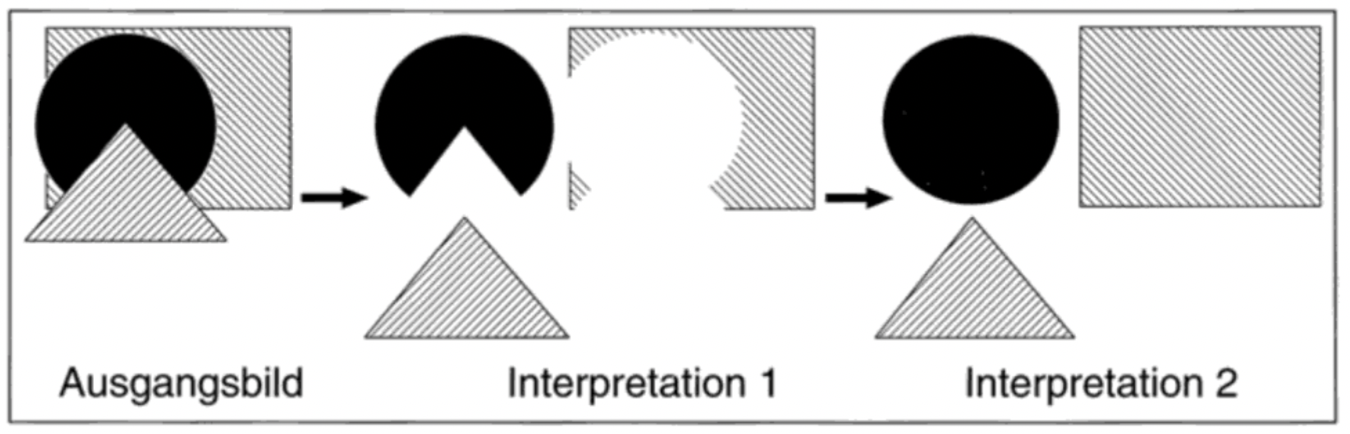
\includegraphics[width=0.8\textwidth]{img/bild_interpretation.jpg}
	\caption{Interpretation einer CT-Aufnahme nach \citet[Seite 360]{lehmann2013bildverarbeitung}}
	\label{fig:interpretation_einer_ct_aufnahem}
\end{figure}

Zu erkennen ist das orginale Bild (Ausgangslage) und mögliche
Interpretationsschritte. \citet[Seite 360]{lehmann2013bildverarbeitung} verdeutlicht
mit dieser Abbildung \ref{fig:interpretation_einer_ct_aufnahem}, dass mittels
orginalem Bild die einzig mögliche Interpretation die erste ist. Auch wenn die zweite
Interpretation die deutlich logischere ist, kann dies ohne weitere Forschung
nicht bewiesen werden, so \citet[Seite 360]{lehmann2013bildverarbeitung}. Für
die Schlussvolgerung von Interpretation 1 auf Interpretation 2 ist eine
Segmentierung des Bildes notwending. Erst mit diesem Verfahren lässt sich zeigen,
wie die Strukturen wirklich aussehen. So beweist dieses Bild, dass die
Segmentierung ein wesentlicher Teil der Bildanalyse ist.

Um ein Bild zu segmentieren gibt es unzählige Möglichkeiten. Für die auswhal eines
Verfahrens spielt der Anwendungsbereich eine wichtige Rolle. Die Verfahren, die in
dieser Arbeit von Wichtigkeit sind, sind die Schwellwertverfahren
\citep[vgl.][Seite 361]{lehmann2013bildverarbeitung}.

\textbf{Schwelltwertverfahren} (engl.: thresholding) gehören zu den Standardwerkzeugen
einer Segmentierung, sodass sie dei Basis vieler weiterer Verfahren legen. Bei
einer Schwellwertbasierten Segmentierung werden die Pixel eines Bildes anhad von
Schwellwerten eingruppiert \citep[vgl.][Seite 96]{handels2000}. Die nachfolgende
Gleichung \ref{equ:schwellwertverfahren} soll dies verdeutlichen.

\begin{align}
	\label{equ:schwellwertverfahren}B(x, y, z) = \begin{cases}1,&\text{falls }t_{\text{unten}}\leq f(x, y, z) \leq t_{\text{oben}}, \\ 0,&\text{sonst}.\end{cases}
\end{align}

$B(x, y, z)$ Beschreibt einen Pixel in einem dreidimensonalen Bild, demnach ein Voxel.
Liegen die Werte eines Voxels, also $f(x, y, z)$ innerhalb der beiden Schwellwerte
$t_{o}ben$ und $t_{u}nten$, dann wird eine 1 zugewiesen. Liegt der aktuell betrachtete
Voxel nicht zwischen den Schwellwerten, so wird eine 0 zugewiesen.

\begin{figure}[h]
	\centering
	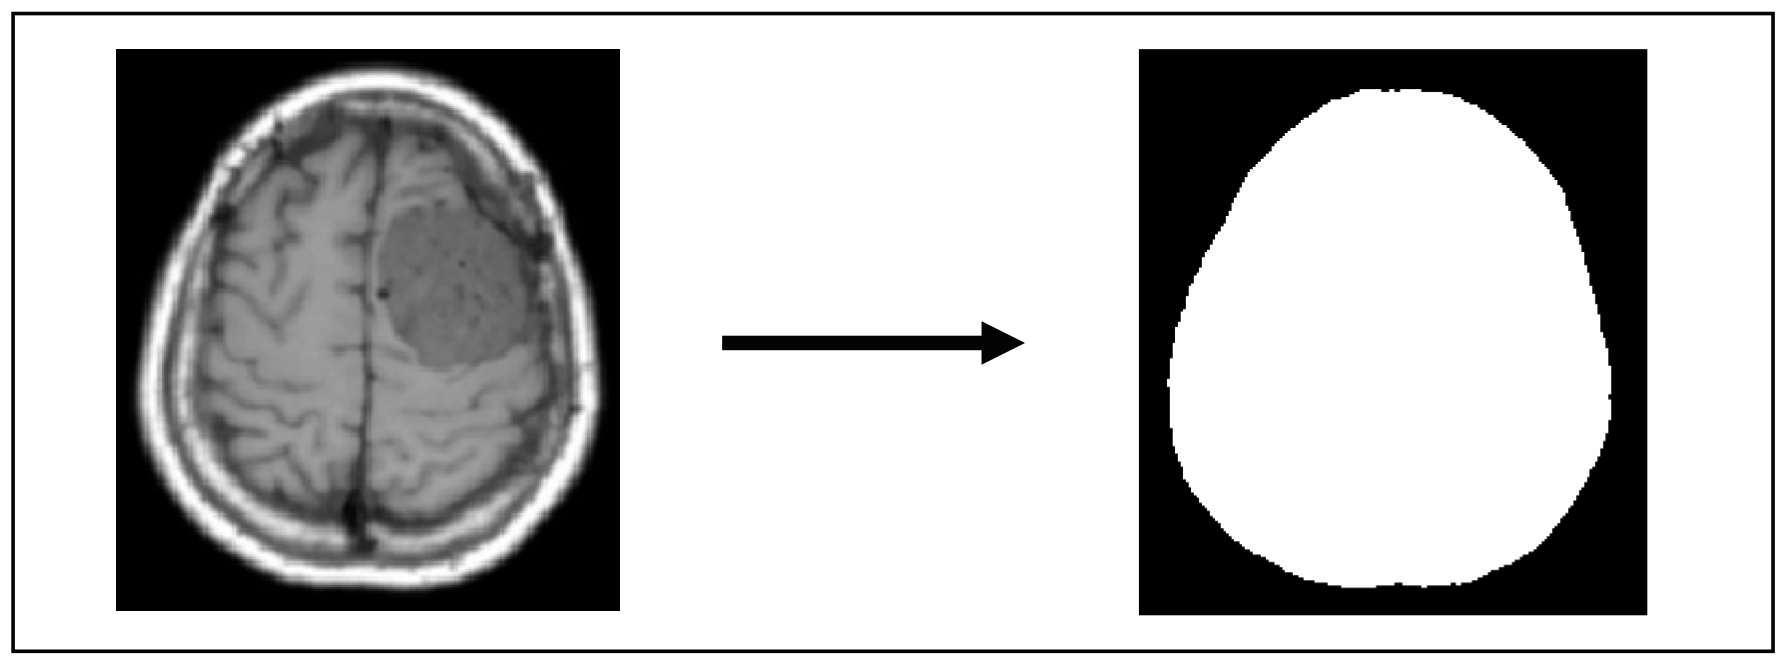
\includegraphics[width=0.8\textwidth]{img/beispiel_schwellwertverfahren.jpg}
	\caption{Ergebnis eines einfachen Schwellwertverfahrens nach \citet[Seite 96]{handels2000}}
	\label{fig:binäres_schwellwertverfahren}
\end{figure}

In der Abbildung \ref{fig:binäres_schwellwertverfahren} ist zu erkennen, dass
nach einem einfachen Schwellwertverfahren das Bild nur noch aus zwei
unterschiedlichen Graustufen besteht. Abgesehen von der Sinnhaftigkeit, ist diese
einfach Segmentierung durchaus erfolgreich verlaufen. Der Grund dafür ist die gute
Wahl des Schwellwertes.

Die interessanteste Frage bei den Schwellwertverfahren ist die Wahl des Schwellwertes $t$.
Diese entscheident zwischen einer guten und einer schlechten Segmentierung. Für die Wahl
eines Schwellwertes empfielt sich der Blick auf das Bildhistogramm. Diese gibt Aufschluss
über die Grauwertverteilung eines Bildes\citep[vgl.][Seite 361]{lehmann2013bildverarbeitung}.
Eines Verfahren, welches eine gute Schwellwertwahl gewährleistet, ohne das zu viele
Informationen verloren gehen, ist das Verfharen nach \textit{Otsu}.

\textbf{Das Verfahren nach Otsu} gehört zu den Schwellwertverfahren und und bestimmt den
Schwellwert $t$ durch ein statistische Gütekriterieum.

\section{Verwandte Arbeit}
\label{sec:verwwandte_arbeit}

\section{Interaktive Bearbeitung mit 3D Slicer}
\label{sec:3d_slicer}
\subsection{Extention Manager}
\subsection{Python Umgebung}
\subsection{MRML Datenstruktur}
\subsection{Qt-Designer}

\section{Architektonisch}
\label{sec:architektonisch}